\SectionNote{presented with homogeneous Dirichlet boundary conditions}
\Section{Presentation}

\begin{frame}{Pipeline of the hybrid method\myfootcite{Ours2026}}
	\centering
	\only<1>{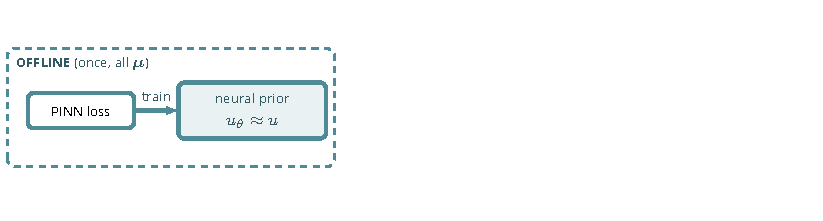
\includegraphics[page=1]{images/contrib1/pipeline/pipeline.pdf}}%
	\only<2-3>{\includegraphics[page=2]{images/contrib1/pipeline/pipeline.pdf}}%
	\only<4>{\includegraphics[page=3]{images/contrib1/pipeline/pipeline.pdf}}%

	\vspace{10pt}
	\raggedright
	\textbf{Offline:} train a \coloredonly<1>{parametric PINN} $u_\theta(\bm{x},\bm{\mu})$ once, for all $\bm{\mu}\in\mathcal{M}$.

	\vspace{6pt}
	\blk{2}{%
		\textbf{Online ($\bm{\mu}$ fixed):} evaluate the prior and its derivatives, solve the \coloredonly<2>{enriched FE} problem.
	}

	\vspace{6pt}
	\blk{3}{%
		\textbf{Goal:} accuracy of a fine mesh on a \coloredonly<3>{coarser mesh}.
	}

	\vspace{6pt}
	\blk*{4}{%
		\textbf{Two versions of} $u_{h,\theta}$\textbf{:} \qquad \coloredonly<4>{additive} $u_{h,\theta}^+$ \quad and \quad \coloredonly<4>{multiplicative} $u_{h,\theta}^\times$.
	}
\end{frame}

\begin{frame}{Additive approach\myfootcite{Ours2026}}
	\begin{minipage}[t]{0.64\linewidth}
		\vspace{0pt}
		\textbf{Prior:} \quad Let $u_{\theta}\in H^{k+1}(\Omega)$ be the PINN prediction (\coloredonly<1>{$\bm{\mu}$ fixed}).

		\vspace{6pt}
		\blk{2}{%
		\textbf{Enriched trial space:}
		\vspace{-3pt}
		\[
			V_h^+=\big\{ \coloredonly<2>{u_{h,\theta}^+=u_{\theta}+p_h^+},\quad p_h^+\in V_h^0\big\}
		\]
		}

		\vspace{6pt}
		\blk{3}{%
			\textbf{Variational problem:} \quad Find $p_h^+\in V_h^0$ such that, $\forall v_h\in V_h^0$,
			\vspace{-3pt}
			\[
				a(p_h^+,v_h)=l(v_h)-\coloredonly<3>{a(u_{\theta},v_h)}\tag{$\mathcal{P}_h^+$}
			\]
			with modified Dirichlet BC. \qquad \refappendix{bc}
		}

		\vspace{8pt}
		\only<4>{%
			\centering
			\textcolor{darkred}{\textbf{Same results as the standard FEM on coarser meshes.}}
		}
	\end{minipage} \hfill \begin{minipage}[t]{0.32\linewidth}
		\vspace{0pt}
		\centering
		\only<1>{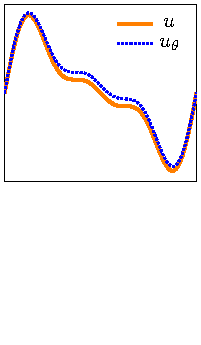
\includegraphics[page=1]{images/contrib1/prior/prior.pdf}}%
		\only<2->{\includegraphics[page=2]{images/contrib1/prior/prior.pdf}}

	\end{minipage}
\end{frame}

\begin{frame}{Multiplicative approach\myfootcite{Ours2026}}
	\textbf{Lifted problem:} \quad $u_M=u+M>0$, with $M\in\mathbb{R}_+$ a constant, solves
	\vspace{-3pt}
	\[
		\left\{\begin{aligned}
			\mathcal{L}(u_M) & = f &  & \text{in } \Omega, \\
			u_M              & = M &  & \text{on } \Gamma,
		\end{aligned}\right.
		\qquad \text{so that } u=u_M-M.
	\]

	\vspace{4pt}
	\blk{2}{%
		\textbf{Lifted prior:} \quad $u_{\theta,M}=u_\theta+M$ \coloredonly<2>{never vanishes}.
	}

	\vspace{6pt}
	\blk{3}{%
	\textbf{Enriched trial space:}
	\[
		V_h^\times=\big\{\coloredonly<3>{u_{h,\theta}^\times=u_{\theta,M}\,p_h^\times-M},\quad p_h^\times\in 1+V_h^0\big\}
	\]
	% Enriched basis: $\phi_i^\times=u_{\theta,M}\,\phi_i$.
	}

	\vspace{6pt}
	\blk{4}{%
		\textbf{Variational problem:} \quad Find $p_h^\times\in 1+V_h^0$ such that, $\forall v_h\in V_h^0$,
		\vspace{-3pt}
		\[
			a\big(u_{\theta,M}\,p_h^\times,u_{\theta,M}\,v_h\big)=l\big(u_{\theta,M}\,v_h\big)\tag{$\mathcal{P}_h^\times$}
		\]
		with modified Dirichlet BC. \qquad \refappendix{bc}
	}

	% \vspace{8pt}
	% \blk*{4}{%
	% 	\textbf{Basis = prior $\times$ Lagrange:} \coloredonly<4>{same structure} as the 2nd hybridization ($m_\theta\,\phi_i$).
	% }

	\vspace{8pt}
	\only<5>{%
		\centering
		\textcolor{darkred}{\textbf{Same results as the standard FEM on coarser meshes.}}
	}
\end{frame}

\begin{frame}{Convergence analysis\footnote[frame,1]{Stated in $L^2$ norm; similar result in $H^1$ semi-norm.}}
	\setcounter{tcb@cnt@mytheo}{0}
	\hypersetup{
		citecolor=white,
	}

	\vspace{-10pt}

	\begin{mytheo}{Standard FEM \footnotesize\parencite{Ern2004}\normalsize}{fem}
		Let $u_h\in V_h^0$ be the solution of the standard FEM. Then,
		\vspace{-3pt}
		\[
			\| u-u_h\|_{L^2} \leqslant C_{L^2} \, h^{k+1} |u|_{H^{k+1}}.
		\]
	\end{mytheo}

	\only<2-3>{\vspace{-4pt}\begin{mytheo}{Additive approach \footnotesize\parencite{Ours2026}\normalsize}{add}
			Let $u_{h,\theta}^+\in V_h^+$ be the solution of ($\mathcal{P}_h^+$) with $V_h^+$ the enriched trial space. Then,
			\vspace{-3pt}
			\[
				\| u-u_{h,\theta}^+\|_{L^2} \leqslant \fcolorbox{orange}{other!10!white}{$C_{\text{gain}}^{+}$} \left(C_{L^2} \, h^{k+1} |u|_{H^{k+1}}\right).
			\]
		\end{mytheo}}

	\hypersetup{
		citecolor=other,
	}

	\only<3>{%
	\centering
	\large $\fcolorbox{orange}{white}{$\displaystyle C_{\text{gain}}^{+}=\frac{| u-u_{\theta} |_{H^{k+1}}}{| u |_{H^{k+1}}}$} < 1 \;\Rightarrow\;$ \textcolor{darkred}{\textbf{gain over the standard FEM}}
	}

	\hypersetup{
		citecolor=white,
	}

	\only<4->{\addtocounter{tcb@cnt@mytheo}{1}\vspace{-4pt}\begin{mytheo}{Multiplicative approach \footnotesize\parencite{Ours2026}\normalsize}{mult}
			Let $u_{h,\theta}^\times\in V_h^\times$ be the solution of ($\mathcal{P}_h^\times$) with $V_h^\times$ the enriched trial space. Then,
			\vspace{-3pt}
			\[
				\| u-u_{h,\theta}^\times\|_{L^2} \leqslant \fcolorbox{red}{other!10!white}{$C_{\text{gain}}^{\times,M}$} \left(C_{L^2} \, h^{k+1} |u|_{H^{k+1}}\right).
			\]
		\end{mytheo}}

	\hypersetup{
		citecolor=other,
	}

	\only<5->{%
	\centering
	\normalsize $\fcolorbox{red}{white}{$\displaystyle C_{\text{gain}}^{\times,M}=C_{\theta,M}\left| \frac{u_M}{u_{\theta,M}} \right|_{H^{k+1}} \frac{\| u_{\theta,M}\|_{W^{1,\infty}}^2}{| u |_{H^{k+1}}}$} < 1 \;\Rightarrow\;$ \textcolor{darkred}{\textbf{gain over the standard FEM}}

	\centering
	\small with $C_{\theta,M}=\|u_{\theta,M}^{-1}\|_{L^{\infty}}+2|u_{\theta,M}^{-1}|_{W^{1,\infty}}+|u_{\theta,M}^{-1}|_{W^{2,\infty}}$ %\;\refappendix{gain}
	}
\end{frame}

\begin{frame}{Multiplicative versus additive\footnote[frame,1]{Stated in $L^2$ norm; similar result in $H^1$ semi-norm.}}
	\setcounter{tcb@cnt@mytheo}{3}
	\hypersetup{
		citecolor=white,
	}

	\begin{mytheo}{Comparison of the gains \footnotesize\parencite{Ours2026}\normalsize}{comp}
		The multiplicative gain converges to the additive gain when $M\to\infty$:
		\vspace{-3pt}
		\[
			\fcolorbox{red}{other!10!white}{$C_{\text{gain}}^{\times,M}$}
			\;\underset{M\to\infty}{\longrightarrow}\;
			\fcolorbox{orange}{other!10!white}{$C_{\text{gain}}^{+}$}
		\]
	\end{mytheo}

	\hypersetup{
		citecolor=other,
	}

	\only<2->{%
		\vspace{10pt}
		\centering
		\large \textcolor{darkred}{\textbf{$M\to\infty$: multiplicative $\to$ additive}} %\;\refappendix{gain}
	}
\end{frame}
